\documentclass{article}

\usepackage{fancyhdr}
\usepackage{extramarks}
\usepackage{amsmath}
\usepackage{amsthm}
\usepackage{amsfonts}
\usepackage{tikz}
\usepackage{graphicx}
\usepackage{enumitem}
\usepackage[plain]{algorithm}
\usepackage{algpseudocode}
\usepackage[normalem]{ulem}
\usepackage{hyperref}
\usepackage{xcolor}
\usepackage{caption}
\usepackage{subcaption}
\usepackage{listings}% http://ctan.org/pkg/listings
\lstset{
  basicstyle=\ttfamily,
  mathescape
}

\hypersetup{
    colorlinks=true,
    linkcolor=blue,
    filecolor=magenta,      
    urlcolor=blue,
}
 
\usetikzlibrary{automata,positioning}

\topmargin=-0.45in
\evensidemargin=0in
\oddsidemargin=0in
\textwidth=6.5in
\textheight=9.0in
\headsep=0.25in

\linespread{1.1}

\pagestyle{fancy}
\lhead{\hmwkAuthorName}
\rhead{\hmwkClass\: \hmwkTitle}
% \rhead{\firstxmark}
\lfoot{\lastxmark}
\cfoot{\thepage}

\renewcommand\headrulewidth{0.4pt}
\renewcommand\footrulewidth{0.4pt}

\setlength\parindent{0pt}

\setcounter{secnumdepth}{0}
\newenvironment{homeworkProblem}[1][-1]{
    \ifnum#1>0
        \setcounter{homeworkProblemCounter}{#1}
    \fi
    \section{Problem \arabic{homeworkProblemCounter}}
    \setcounter{partCounter}{1}
    \enterProblemHeader{homeworkProblemCounter}
}{
    \exitProblemHeader{homeworkProblemCounter}
}

\newcommand{\hmwkTitle}{Project Proposal}
\newcommand{\hmwkClass}{CSE 403 (Wi16)}
\newcommand{\hmwkAuthorName}{Ryan Drapeau | Sonja Khan}
\newcommand{\hmwkAuthorCSE}{drapeau@cs.washington.edu}

\title{
    \vspace{2in}
    \textmd{\textbf{\hmwkClass:\ \hmwkTitle}}\\
    \vspace{0.1in}\large{\textit{\hmwkClassInstructor\ \hmwkClassTime}}\\
    \author{\textbf{\hmwkAuthorName\ $\vert$ \hmwkAuthorCSE\ $\vert$ \hmwkAuthorId}}
}

\date{}

\renewcommand{\part}[1]{\textbf{\large Part \Alph{partCounter}}\stepcounter{partCounter}\\}

\DeclareMathOperator*{\argmin}{arg\,min}

\DeclareMathOperator*{\argmax}{arg\,max}

\begin{document}

\pagebreak

\begin{minipage}{\linewidth}
    \centering
    
\includegraphics[width=0.80\textwidth]{logo.jpg}
\end{minipage}

\subsection{Overview}

With the 2016 presidential race well under way, the media has had a profound effect on the public's perception of each candidate. As the race continues to narrow down to only a few presidential candidates, it is becoming increasingly important that people understand the values and views each candidate would bring as president. However, major issues exist with the political system in America. One problem being that many sources for campaign news can be incredibly biased, especially when a candidate's campaign is being funded by the news organization. Another issue is the lack of young voters in America. We propose an app, named \textbf{Check Your Bias} (CYB), that aims to help combat these problems.\\

CYB is a mobile application where users will respond to quotes, topics, and issues by using a sliding scale to indicate if they ``Agree'' or ``Disagree''. Some topics may include economy, gun control, immigration, etc. The novel feature of CYB is that there is no indication of which candidate supports or opposes the presented issue, removing the bias that the user may of had if they had known a candidate's position. After submitting a response, the user has the option to see where they stand in relation to other candidates' positions. Some users may find that their stance on an issue falls more closely towards a candidate they had no intention in voting for.\\ 

This process of presenting issues and subsequently showing candidates' positions removes any candidate bias the user may have had if they had known the positions when voting. The application flow also serves to educate users on important issues or policies by also including relevant news articles on the same view that shows the positions. This also has the effect that someone might change their stance on a topic after reading current news becoming more informed.
\vspace{-5px}
\subsection{Related Work}

The most related pieces of work consist of the main news applications and organizations that are covering the 2016 presidential campaign. Some noteworthy apps include \href{http://www.cnn.com/politics}{CNN}, \href{http://www.nbcnews.com/politics/2016-election}{NBCNews}, \href{http://live.reuters.com/Event/Election_2016?Page=64}{Reuters}, and several more. The main difference between CYB and news applications is the anonymity of the candidates' positions in the presentation of the issue. For example, CNN recently published an article titled ``Trump jokingly reprimands supporters in New Hampshire''. Before a reader even begins the article, they have a predisposition to favoring or opposing the article simply because of the candidate mentioned. Instead, CYB will help users become more informed on where they might stand on issues and which candidates share those views with them. 
\vspace{-5px}
\subsection{Risks}

A big issue that could impede the development of this application is: how is the content (the topics, issues, candidate positions, etc.) generated? We aim to solve this problem with the users of the application. We will implement a form of crowdsourcing that allows users to submit content, which will then be displayed to other users' feeds. Submitted content can be verified in many ways to ensure the authenticity of the source. If the source is submitted many times by different users, then it is more likely that the source is accurate and can be used in the app's content database.\\

However, the system will need to have data pre-populated before the first user downloads the application. This can be mitigated by generating content ($>$ 50 topics) by hand before the app's release. Another issue could be that some topics or quotes have multiple instances in the database. This problem can also be reduced using a crowdsourcing functionality by simply having a ``I've already seen this'' option when a user is evaluating a piece of content. 

\begin{figure}[t]
\begin{center}
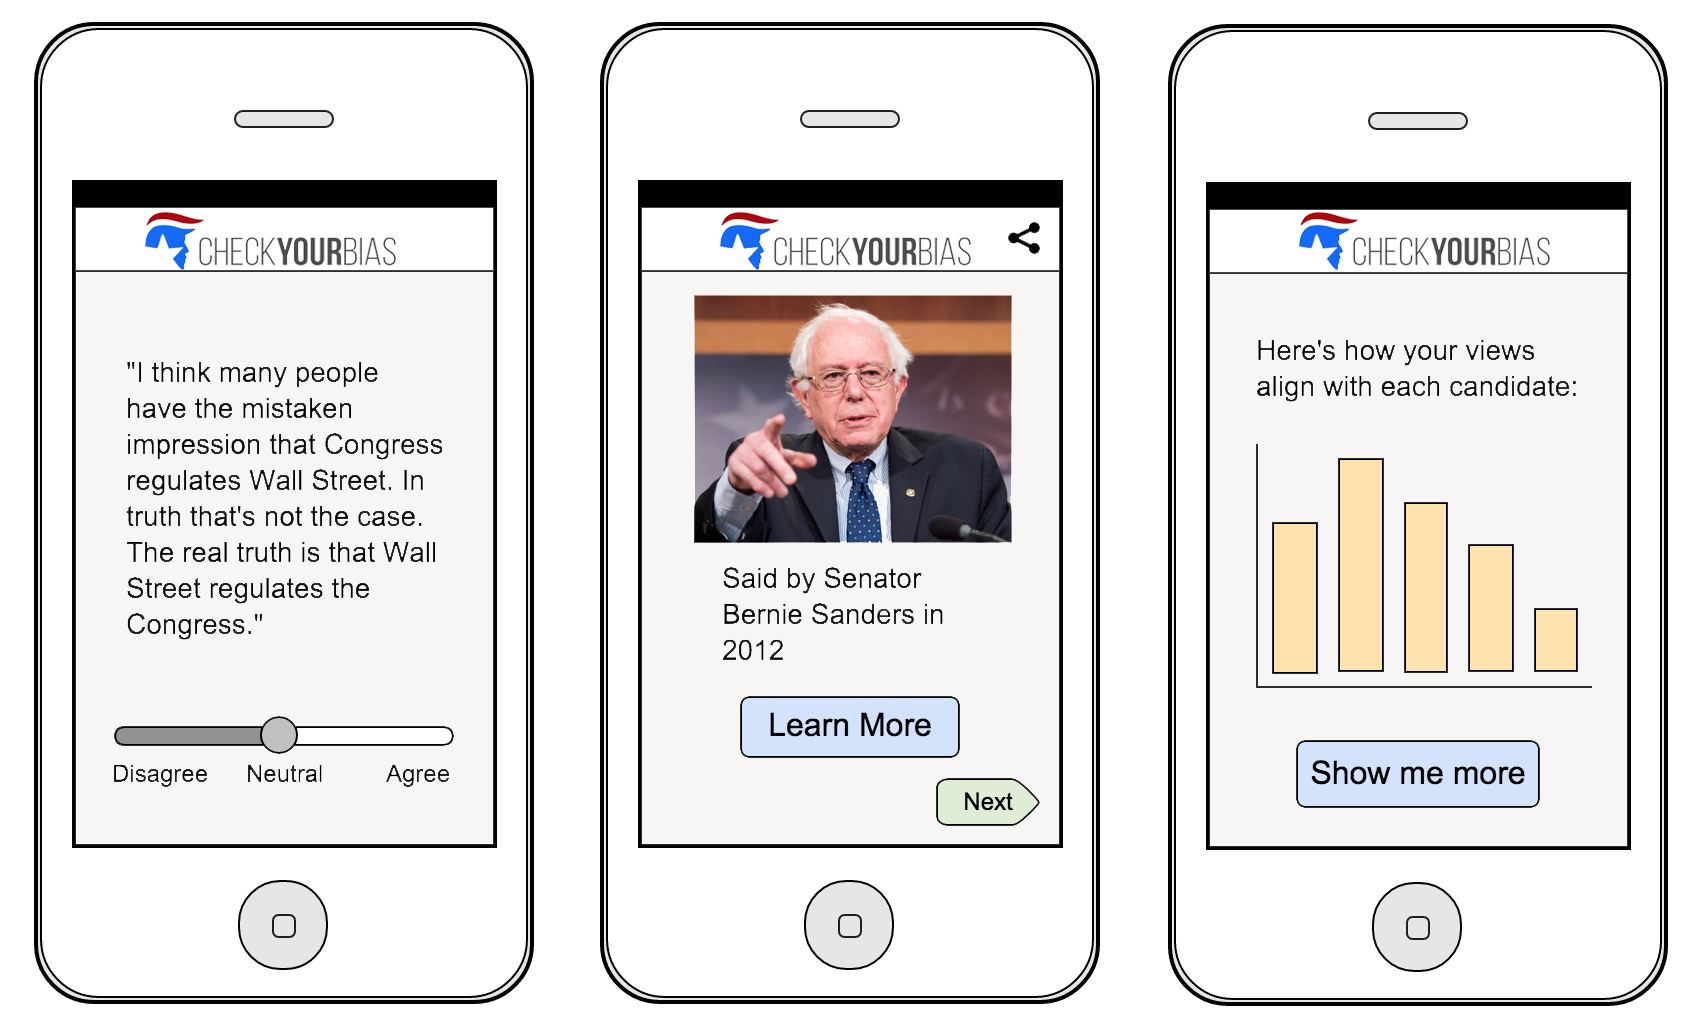
\includegraphics[width=0.95\textwidth]{mock.png}
\vspace*{-0.05in}
\caption{Mockup of the 3 main views of CYB. \textbf{Left}: The user can decide their stance to an issue/quote/topic. \textbf{Middle}: The user is shown the candidate that said the quote or candidates that have a similar position as the user. \textbf{Right}: An analysis view ranks the candidates according to how closely the user's views align with candidates' views.}
\label{fig:mock}
\end{center}
\vspace{-0.2in}
\end{figure}

\subsection{Implementation Details}

This project will be implemented using \href{http://phonegap.com/}{PhoneGap}, a library that specializes in creating cross-platform applications using HTML, CSS, and Javascript. This removes most of the nuances of developing for Android or iOS and replaces them with web development tools. Facebook's \href{https://facebook.github.io/react/}{React} will be used to design the user interfaces and will prove to be extremely useful with binding the content and data to the view. The majority of the crowdsourcing experimentation and computation will take place on the backend so that users will only need to submit content in order for it to be approved for use in the application. Different crowdsourcing techniques will be explored, ranging from majority vote to peer approval in order to verify the submitted content. CYB also requires a sophisticated back end server that will provide the content in the application, which means that CYB must be connected to the Internet in order to function correctly.

\subsection{Conclusion}

We have presented a novel application, \textbf{Check Your Bias}, that will help address the issue of bias in the 2016 political campaign. CYB contains many distinct features (slider, content creation, candidate stance, related news, etc.), which can easily be assigned to developers or subteams to complete in parallel during the course of CSE 403. 

\end{document}
